\documentclass[11pt]{article}

\usepackage[a4paper,margin=1in]{geometry}
\usepackage{amsmath}
\usepackage{amssymb}
\usepackage{booktabs}
\usepackage{tabularx}
\usepackage{graphicx}
\usepackage[hidelinks]{hyperref}
\usepackage[authoryear,round]{natbib}
\usepackage{siunitx}
\usepackage{tikz}
\usetikzlibrary{arrows.meta,positioning}
\sisetup{group-separator={,}, group-minimum-digits=4}

\title{Class Imbalance Mitigation:\\
Methods and Evaluation Framework}
\author{Yannik Queisler}
\date{\today}

\begin{document}
\maketitle

\begin{abstract}
\noindent Class imbalance in computational pathology depends on the input regime: labeled image patches support ordinary classification, whereas whole-slide image (WSI) diagnosis is commonly modeled as weakly supervised learning over patch-feature bags. This report introduces representative class-imbalance mitigation methods for histopathology classification and the framework used to evaluate them. The methods are organized by the level at which they intervene---data-level sampling and augmentation, algorithm-level losses, hybrid sampling--loss objectives, synthetic generation, and representation or architecture-level methods---and are described in the input form each is designed to consume, with cross-entropy as the no-mitigation reference. The evaluation framework then defines the discrimination metrics used for ranking (macro F1, balanced accuracy, and class-group recall) and the probability-quality metrics used to check whether reported confidences are trustworthy (negative log likelihood, multiclass Brier score, and expected calibration error, before and after a unified post-hoc temperature-scaling protocol).
\end{abstract}

\setcounter{tocdepth}{2}
\tableofcontents
\clearpage

\section{Introduction}
Class imbalance changes what a pathology classifier is rewarded for learning. When common tumor types dominate training data, high aggregate accuracy can coexist with unreliable rare-class recall, especially if evaluation emphasizes prevalence-sensitive metrics. Long-tailed learning and medical-image evaluation literature therefore motivate classwise recall, macro F1, balanced accuracy, and calibration-aware probability metrics as primary outcomes in imbalanced settings \citep{saini2023tacklingClass,zhang2023deepLong,mosquera2024classImbalance}.

Imbalance methods often assume a specific prediction unit. Image-level methods use labeled images, image embeddings, or directly generated image samples, whereas WSI-level methods use weak labels over bags of instances together with attention, instance ranking, or bag-level representation learning. Each method family is therefore described in the input form it is designed to consume. The broader computational-pathology pipeline these regimes sit in---whole-slide imaging, patching into tiles, and weakly supervised multiple-instance learning over frozen foundation-model features---is introduced in the companion datasets report \citep{queisler2026datasets}.

This report has two purposes. Section~\ref{sec:methods} introduces the class-imbalance mitigation methods themselves, organized by the level at which they intervene and stated in enough mathematical detail to make the imbalance mechanism explicit. Section~\ref{sec:evaluation} then introduces the evaluation framework: the discrimination metrics used to rank methods and the probability-quality metrics used to judge whether their reported confidences are trustworthy. The aim is not to introduce a new mitigation method, but to fix the method definitions and evaluation protocol used when instantiating these methods on specific pathology datasets.

\paragraph{Prediction regimes.}
The methods are described for two prediction regimes that recur throughout the benchmarks. In the \emph{patch} regime, each labeled crop is an independent example: a frozen foundation-model encoder such as Virchow2 embeds the patch once, and a lightweight classifier head is trained on the resulting embedding \citep{zimmermann2024virchow2,vorontsov2024virchow}. In the \emph{WSI-bag} regime, a slide is represented as a bag of frozen patch-feature instances that share one weak slide-level label, and an attention-based multiple-instance-learning (MIL) head aggregates the instances into a slide prediction. Both regimes rely on the same pathology foundation-model family and therefore consume the same embeddings; they differ only in supervision unit---one embedding per selected patch versus aggregation over a bounded set of instances on a slide. Freezing the encoder isolates the imbalance mechanism from end-to-end backbone learning, so method differences within a regime correspond to imbalance interventions rather than to changes in encoder, features, or evaluation code. Each non-baseline method exposes one imbalance-specific control (for example the focal focusing parameter, the CFAL affinity bandwidth, or the RankMix mixing parameter); the concrete validation grids and the values selected on each dataset are reported in the companion experiment reports.

\section{Methods}
\label{sec:methods}
The methods are organized by the level at which they intervene in the imbalanced learning problem. Cross-entropy (CE) is treated as the no-mitigation reference condition: it uses the observed training distribution as given and does not rebalance samples, labels, costs, representations, or generated data. The remaining methods are imbalance interventions grouped according to the taxonomy used in the class-imbalance literature: data-level sampling and augmentation, algorithm-level losses, hybrid sampling--loss methods, synthetic generation, and representation or architecture-level methods \citep{saini2023tacklingClass,zhang2023deepLong}.

The comparison is regime-specific. Patch methods consume frozen Virchow2 embeddings of controlled patches and optimize one shared MLP classifier head; CE-based patch methods use the same linear output layer, while CFAL replaces that layer with class prototypes and affinity-based prediction. WSI-bag methods consume capped frozen Virchow2 feature bags and optimize one shared attention-MIL head. Both regimes therefore rely on the same pathology foundation-model family, but they differ in supervision unit: one embedding per selected patch versus aggregation over a bounded set of instances on a slide.

\begin{figure}[ht]
  \centering
  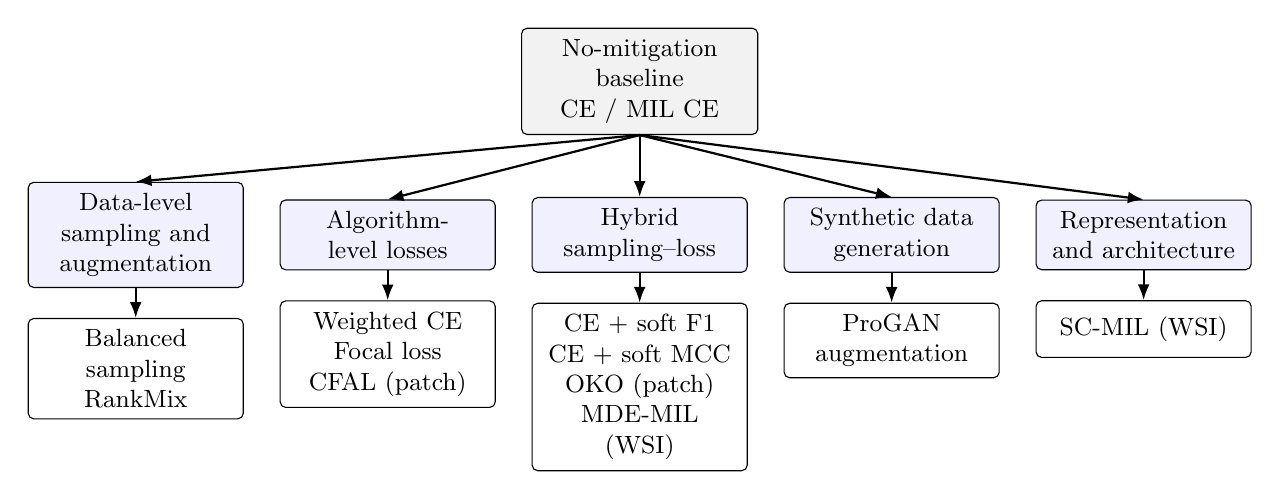
\begin{tikzpicture}[
    box/.style={draw, rounded corners=2pt, align=center, inner sep=4pt, font=\small, minimum height=0.72cm},
    baseline/.style={box, fill=gray!10, minimum width=3.0cm},
    family/.style={box, fill=blue!6, text width=2.45cm},
    method/.style={box, fill=white, text width=2.45cm},
    arrow/.style={-{Latex[length=2mm]}, thick}
  ]
    \node[baseline] (ce) at (0,0) {No-mitigation\\baseline\\CE / MIL CE};
    \node[family] (data) at (-6.4,-1.95) {Data-level sampling and augmentation};
    \node[method, below=0.38cm of data] (dataMethods) {Balanced sampling\\RankMix};
    \node[family] (loss) at (-3.2,-1.95) {Algorithm-level losses};
    \node[method, below=0.38cm of loss] (lossMethods) {Weighted CE\\Focal loss\\CFAL (patch)};
    \node[family] (hybrid) at (0,-1.95) {Hybrid sampling--loss};
    \node[method, below=0.38cm of hybrid] (hybridMethods) {CE + soft F1\\CE + soft MCC\\OKO (patch)\\MDE-MIL (WSI)};
    \node[family] (synthetic) at (3.2,-1.95) {Synthetic data generation};
    \node[method, below=0.38cm of synthetic] (syntheticMethods) {ProGAN\\augmentation};
    \node[family] (repr) at (6.4,-1.95) {Representation and architecture};
    \node[method, below=0.38cm of repr] (reprMethods) {SC-MIL (WSI)};
    \draw[arrow] (ce.south) -- (data.north);
    \draw[arrow] (ce.south) -- (loss.north);
    \draw[arrow] (ce.south) -- (hybrid.north);
    \draw[arrow] (ce.south) -- (synthetic.north);
    \draw[arrow] (ce.south) -- (repr.north);
    \draw[arrow] (data) -- (dataMethods);
    \draw[arrow] (loss) -- (lossMethods);
    \draw[arrow] (hybrid) -- (hybridMethods);
    \draw[arrow] (synthetic) -- (syntheticMethods);
    \draw[arrow] (repr) -- (reprMethods);
  \end{tikzpicture}
  \caption{Method organization used in the benchmarks. Cross-entropy is the no-mitigation reference, while the tested alternatives intervene through sampling, loss design, synthetic data, WSI feature augmentation, or representation learning.}
  \label{fig:method-taxonomy}
\end{figure}

\subsection{Notation}
Let $C$ be the number of cancer-type classes and let $n_c$ denote the number of training examples from class $c$. For a labeled patch or slide-level bag with label $y\in\{1,\ldots,C\}$, the model outputs logits $\mathbf{z}\in\mathbb{R}^{C}$ and class probabilities
\begin{equation}
  p_c = \frac{\exp(z_c)}{\sum_{j=1}^{C}\exp(z_j)}.
  \label{eq:softmax}
\end{equation}
For WSI-bag methods, a slide is represented as a bag $B=\{\mathbf{x}_1,\ldots,\mathbf{x}_m\}$ of frozen patch-feature instances. The attention-MIL backbone maps each bag to a bag embedding $\mathbf{b}(B)$ and class logits. Unless a method explicitly changes the sampler, objective, or representation loss, the empirical class frequencies in the training set define the optimization signal.

\subsection{Cross-Entropy Baseline}
Unweighted cross-entropy is the baseline because it is the standard supervised objective without an explicit class-imbalance correction. For an example with label $y$, the loss is
\begin{equation}
  \mathcal{L}_{\mathrm{CE}}(\mathbf{z},y) = -\log p_y.
  \label{eq:ce}
\end{equation}
In the patch regime, this objective trains the shared linear head on frozen Virchow2 patch embeddings from the controlled manifest. In the WSI-bag regime, the same objective trains the shared attention-MIL model on slide-level feature bags. In both cases, CE uses the observed class distribution directly: majority classes appear more often in minibatches and therefore contribute more loss terms over an epoch. This makes CE an appropriate reference for asking whether an imbalance-specific intervention actually improves the rare-class tradeoff.

\subsection{Data-Level Sampling and Augmentation}
Data-level methods change what the optimizer sees, rather than changing the mathematical penalty assigned to one observed example. In the taxonomy, this family includes resampling, augmentation, and WSI-specific feature mixing strategies that make minority or informative examples more visible during training \citep{saini2023tacklingClass}.

\subsubsection{Balanced Sampling}
Balanced sampling changes minibatch composition by sampling training examples with probabilities inversely related to their class support. For an example $i$ with class $y_i$, the sampler weight is proportional to
\begin{equation}
  q_i \propto \frac{1}{n_{y_i}}.
  \label{eq:balanced-sampling}
\end{equation}
After normalization across the training set, this makes the expected class exposure closer to uniform even though the underlying dataset remains imbalanced. The patch variant applies this sampler to patch examples and still optimizes CE. The MIL variant applies the same idea at slide-bag level and also optimizes CE. Balanced sampling therefore tests a pure data-level intervention: it asks whether equalizing training exposure is enough without changing the loss formula.

\subsubsection{RankMix}
RankMix is a WSI-native data-augmentation method for weakly supervised slide classification. Ordinary image mixup assumes two inputs with compatible spatial shapes, but WSI bags can contain different numbers of feature instances and lack instance-level labels. RankMix addresses this by mixing representative feature subsequences rather than raw slides \citep{chen2023rankmix}.

The tested implementation follows the defining two-stage teacher--student procedure. First, a teacher attention-MIL model is trained with slide labels for 30 epochs using the same MIL architecture and optimization settings as plain MIL CE. For each bag $B=\{\mathbf{x}_1,\ldots,\mathbf{x}_m\}$ and target class, the teacher assigns ranking scores to instances using its softmax probability for that class; the top-$k$ instances are kept as a representative subsequence, where $k=\min(|B_a|,|B_b|)$ for the two bags being mixed, and their original within-bag order is preserved after selection. The student MIL model is then reinitialized and trained on bags built from these ranked subsequences.

Mixing itself follows the mixup idea in feature space. For two bags $a$ and $b$, let $H_a$ and $H_b$ denote the selected instance-feature matrices and $\mathbf{y}_a,\mathbf{y}_b$ the corresponding one-hot slide labels. A scalar mixing coefficient $\lambda\in(0,1)$ controls how much of each bag is retained:
\begin{equation}
  \widetilde{H}=\lambda H_a+(1-\lambda)H_b,
  \qquad
  \widetilde{\mathbf{y}}=\lambda \mathbf{y}_a+(1-\lambda)\mathbf{y}_b.
  \label{eq:rankmix}
\end{equation}
\noindent When $\lambda$ is close to one, the mixed bag resembles bag $a$; when it is close to zero, it resembles bag $b$. Values near $\lambda=\tfrac{1}{2}$ interpolate more evenly between the two sources. RankMix does not fix $\lambda$ to a single value. Instead, each mixed example draws
\begin{equation}
  \lambda \sim \mathrm{Beta}(\alpha,\alpha),
  \label{eq:rankmix-beta}
\end{equation}
\noindent independently. The Beta distribution is a standard choice on the open interval $(0,1)$ because it is flexible and symmetric when both shape parameters are equal. With density
\begin{equation}
  f(\lambda;\alpha,\alpha)\propto \lambda^{\alpha-1}(1-\lambda)^{\alpha-1},
  \qquad \lambda\in(0,1),
  \label{eq:beta-density}
\end{equation}
\noindent the parameter $\alpha>0$ controls how strongly mixing concentrates around the endpoints versus the center. For $\alpha=1$, $\mathrm{Beta}(1,1)$ is the uniform distribution on $(0,1)$, so every mixing weight is equally likely and the procedure reduces to ordinary symmetric mixup. Larger $\alpha$ pushes $\lambda$ toward $\tfrac{1}{2}$, producing more balanced interpolations; smaller $\alpha$ pushes mass toward $0$ and $1$, producing mixtures that stay closer to one source bag. The reference default is $\alpha=\num{1.0}$, matching the RankMix source implementation, and $\alpha$ is the imbalance control selected on validation. The student is trained with soft-label cross-entropy on the mixed bags and labels $\widetilde{\mathbf{y}}$. This mechanism is categorized as data-level augmentation because it increases the diversity of the training bags in feature space while retaining the same attention-MIL prediction architecture.

\subsection{Algorithm-Level Losses}
Algorithm-level methods keep the training examples fixed but alter how errors are penalized. They are cost-sensitive or difficulty-sensitive objectives: minority examples may receive larger explicit weights, or easy examples may contribute less to the gradient \citep{saini2023tacklingClass,scholz2024imbalanceAware}.

\subsubsection{Class-Weighted Cross-Entropy}
Class-weighted CE multiplies each example's CE term by a class-dependent cost:
\begin{equation}
  \mathcal{L}_{\mathrm{WCE}}(\mathbf{z},y) = -w_y\log p_y,
  \qquad
  w_c \propto \frac{1}{n_c}.
  \label{eq:weighted-ce}
\end{equation}
The implementation normalizes the inverse-frequency weights so that the average scale of the loss remains comparable across methods. This method leaves the sample order and model architecture unchanged, but increases the loss contribution of classes with fewer training examples. It is evaluated for both patch classification and attention-MIL.

\subsubsection{Focal Loss}
Focal loss reduces the contribution of confidently classified examples and concentrates optimization on examples that remain difficult. With focusing parameter $\gamma$, the multiclass focal objective is
\begin{equation}
  \mathcal{L}_{\mathrm{focal}}(\mathbf{z},y) =
  -(1-p_y)^{\gamma}\log p_y.
  \label{eq:focal}
\end{equation}
The reference default is $\gamma=\num{2.0}$ for both regimes; $\gamma$ is the imbalance control selected on validation while the rest of the training protocol is held fixed. The method is relevant to imbalance because many minority-class examples can remain hard under a classifier dominated by head-class gradients, but the focal term does not directly encode the class counts. It is therefore a difficulty-sensitive loss rather than a sampler or explicit prior correction.

\subsubsection{Center-Focused Affinity Loss (CFAL)}
Center-focused affinity loss (CFAL) replaces the linear softmax head with learnable class prototypes and an affinity-based training objective \citep{mahbub2024centerFocused}. The motivation is that minority histology classes can remain visually similar in embedding space even when a frozen encoder already separates them coarsely; pulling examples toward compact class centers and penalizing confusion with nearby wrong-class prototypes can therefore improve tail-class boundaries without changing the sampler.

The tested patch implementation keeps the shared MLP trunk that maps a frozen Virchow2 embedding $\mathbf{x}$ to a hidden representation $\mathbf{z}=f(\mathbf{x})\in\mathbb{R}^{512}$, but replaces the final linear map with one learnable prototype $\mathbf{w}_c\in\mathbb{R}^{512}$ per class. Both embeddings and prototypes are L2-normalized before affinity computation. The Gaussian affinity between example $i$ and class $c$ is
\begin{equation}
  a_{ic}=\exp\!\left(-\frac{\|\hat{\mathbf{z}}_i-\hat{\mathbf{w}}_c\|_2^2}{\sigma}\right),
  \qquad
  \hat{\mathbf{v}}=\frac{\mathbf{v}}{\|\mathbf{v}\|_2},
  \label{eq:cfal-affinity}
\end{equation}
\noindent where $\sigma$ controls how quickly affinity decays with prototype distance. At inference, class scores are $\log a_{ic}$ followed by softmax normalization. The affinities $a_{ic}\in(0,1]$ are geometric similarity scores, not class probabilities: they are trained with a margin objective and never optimized to satisfy likelihood or calibration constraints. Applying softmax to $\log a_{ic}$ therefore yields a convenient ranking score for argmax decisions, but it should not be read as a calibrated estimate of $P(y=c\mid \mathbf{x})$ without additional post-hoc mapping.

Training optimizes a margin term on affinities rather than cross-entropy on logits. For batch index $i$ with label $y_i$, define the per-example margin loss
\begin{equation}
  \ell_i=\sum_{c\ne y_i}\max\bigl(0,\, \lambda + a_{ic}-a_{i,y_i}\bigr),
  \label{eq:cfal-margin}
\end{equation}
\noindent which penalizes wrong-class affinities that exceed the true-class affinity by less than margin $\lambda$. A diversity regularizer $R(\mathbf{W})$ encourages prototypes to spread apart by penalizing deviations of pairwise squared distances from their mean. The total objective combines class reweighting, a center-focused local weight, and prototype diversity:
\begin{equation}
  \mathcal{L}_{\mathrm{CFAL}}=
  \frac{1}{B}\sum_{i=1}^{B}
  \frac{1}{E_{y_i}}
  (1-a_{i,y_i})^{\gamma}\,\ell_i
  + R(\mathbf{W}),
  \label{eq:cfal-total}
\end{equation}
\noindent where $E_c$ is the effective number of training examples in class $c$ derived from class count $n_c$ and hyperparameter $\beta$, and $\gamma$ up-weights examples whose true-class affinity remains low. Unlike the CE plus soft-F1 and soft-MCC hybrids, CFAL does not use balanced oversampling: it is categorized as an algorithm-level patch method because it changes the head and loss while keeping the natural training distribution.

The reference defaults are $\lambda=\num{0.1}$, $\beta=\num{0.999}$, and $\gamma=\num{2.0}$ following Mahbub et al.; all three are held fixed and the affinity bandwidth $\sigma$ is the imbalance control selected on validation. The paper's $\sigma=\num{130}$ was calibrated for un-normalized AlexNet FC features; on L2-normalized \num{2560}-dimensional Virchow2 vectors that scale is far too large and collapses all pairwise affinities, so the benchmark evaluates a range matched to the normalized embedding geometry. CFAL is evaluated only in the patch regime because the source method assumes instance-level labels rather than weak slide-level bags.

\subsection{Hybrid Sampling--Loss Methods}
Hybrid methods combine data-level and algorithm-level changes. The Scholz-style patch objectives below adapt the metric-derived losses of Scholz et al.\ for imbalanced medical classification \citep{scholz2024imbalanceAware}. Both tested variants use class-balanced oversampling together with metric-derived losses, so their effect cannot be attributed only to a new loss or only to a new sampler.

\subsubsection{Scholz-Style CE + Soft F1}
The intuition is that CE optimizes the log-probability of the correct class one example at a time, whereas macro F1 evaluates a different object: the balance between precision and recall at class level. Under class imbalance, this distinction matters because a model can reduce CE substantially by fitting frequent classes while still leaving tail-class recall or precision weak.

The obstacle is that ordinary F1 is computed from hard counts after prediction, so it is not directly usable as a gradient-based training loss. The Scholz-style soft-F1 objective replaces those hard counts with probability-weighted counts inside each minibatch. For one class, a confident correct prediction contributes almost one soft true positive, a confident prediction for the wrong class contributes to soft false positives, and low probability on a true class contributes to soft false negatives. Formally, for one-hot labels $y_i$ and predicted probabilities $\hat{y}_i$:
\begin{equation}
  \mathrm{TP}=\sum_i y_i\hat{y}_i,\quad
  \mathrm{FP}=\sum_i (1-y_i)\hat{y}_i,\quad
  \mathrm{FN}=\sum_i y_i(1-\hat{y}_i).
  \label{eq:soft-confusion-f1}
\end{equation}
\noindent These terms keep the familiar meaning of a confusion matrix but make every component differentiable with respect to the model probabilities. They then define soft precision, soft recall, and soft F1:
\begin{equation}
  \mathrm{F1}_{\mathrm{soft}} =
  \frac{2\,\mathrm{precision}_{\mathrm{soft}}\,\mathrm{recall}_{\mathrm{soft}}}
       {\mathrm{precision}_{\mathrm{soft}}+\mathrm{recall}_{\mathrm{soft}}}.
  \label{eq:soft-f1}
\end{equation}
\noindent The multiclass implementation applies this construction separately to each class and averages the resulting classwise terms. This macro-style averaging is the imbalance-aware part: each class contributes one term regardless of how many samples it has in the full dataset. The tested objective does not replace CE completely; it adds the metric-derived term to CE so that optimization still rewards calibrated class probabilities while also pushing the minibatch toward higher macro soft F1:
\begin{equation}
  \mathcal{L}_{\mathrm{CE+F1}} = \mathcal{L}_{\mathrm{CE}} +
  \left(1-\frac{1}{C}\sum_{c=1}^{C}\mathrm{F1}_{\mathrm{soft},c}\right).
  \label{eq:ce-soft-f1}
\end{equation}
\noindent The benchmark trains this loss with balanced sampling on the patch manifest. That design is important for interpretation: the loss tries to optimize a macro-style class metric, while the sampler ensures that tail classes occur often enough in minibatches for their soft-F1 terms to provide a regular training signal.

\subsubsection{Scholz-Style CE + Soft MCC}
The soft-MCC variant uses the same principle as soft F1---replace hard evaluation counts with differentiable probability masses---but starts from the Matthews correlation coefficient (MCC). Whereas F1 for one class depends mainly on that class's positive predictions, MCC is built from the full confusion matrix and therefore reacts to false positives, false negatives, and true negatives at the same time. In binary problems it is often preferred in imbalanced settings because it can remain informative when one class dominates the dataset: accuracy can look high while predictions are still systematically biased, but MCC penalizes both kinds of mistakes jointly.

\paragraph{Binary MCC as a correlation coefficient.}
For one class treated as positive, write TP, TN, FP, and FN for the four confusion-matrix cells. The standard MCC is
\begin{equation}
  \mathrm{MCC} =
  \frac{\mathrm{TP}\cdot\mathrm{TN}-\mathrm{FP}\cdot\mathrm{FN}}
       {\sqrt{(\mathrm{TP}+\mathrm{FP})(\mathrm{TP}+\mathrm{FN})
              (\mathrm{TN}+\mathrm{FP})(\mathrm{TN}+\mathrm{FN})}}.
  \label{eq:binary-mcc}
\end{equation}
\noindent The numerator compares co-occurrence of correct positive and correct negative decisions with co-occurrence of the two error types; the denominator scales by how many examples fall into each margin of the confusion matrix. MCC equals $+1$ for perfect predictions, $0$ for chance-level association, and can become negative when predictions are worse than random. This makes it a correlation-style score rather than a prevalence-weighted rate.

\paragraph{Multiclass MCC in a minibatch.}
For $C$ cancer types, the multiclass extension treats labels and predictions as $C$-dimensional vectors per example. Let $Y\in\{0,1\}^{N\times C}$ be the one-hot label matrix and $\widehat{Y}\in[0,1]^{N\times C}$ the corresponding softmax probabilities, with rows $\mathbf{y}_i$ and $\hat{\mathbf{y}}_i$. Three aggregate quantities describe how mass is distributed inside the batch:
\begin{equation}
  s = \sum_{i=1}^{N}\sum_{c=1}^{C} Y_{ic}\widehat{Y}_{ic},
  \qquad
  t_c = \sum_{i=1}^{N} Y_{ic},
  \qquad
  p_c = \sum_{i=1}^{N} \widehat{Y}_{ic}.
  \label{eq:mcc-components}
\end{equation}
\noindent Here $s$ is the total probability-weighted agreement between labels and predictions: each example contributes $\hat{y}_{i,y_i}$, the predicted mass on its true class. The terms $t_c$ and $p_c$ are the batch totals of true and predicted mass for class $c$. They play the role of marginals in the confusion-matrix calculation. If predictions collapse onto a few head classes, the vector $(p_1,\ldots,p_C)$ becomes skewed even when argmax accuracy looks acceptable; MCC is sensitive to that mismatch because it compares the joint alignment $s$ with what would be expected from the marginals alone.

The multiclass MCC used in training can be written as a normalized covariance between the label matrix and the prediction matrix:
\begin{equation}
  \mathrm{MCC}_{\mathrm{mc}} =
  \frac{Ns - \sum_{c=1}^{C} t_c p_c}
       {\sqrt{N^2 - \sum_{c=1}^{C} p_c^2}\;
        \sqrt{N^2 - \sum_{c=1}^{C} t_c^2}}.
  \label{eq:multiclass-mcc}
\end{equation}
\noindent The numerator $Ns-\sum_c t_c p_c$ increases when true and predicted mass line up example by example and decreases when correct predictions are no better than what the marginal totals would suggest by chance. The two square-root terms measure how spread out the batch-level label totals and prediction totals are across classes; they prevent the score from exploding when one minibatch happens to contain only a few classes. Equation~\eqref{eq:multiclass-mcc} reduces to the familiar binary form in \eqref{eq:binary-mcc} when $C=2$.

\paragraph{Soft MCC loss.}
Hard MCC replaces $\widehat{Y}$ by one-hot argmax predictions, which again blocks gradient-based training. The soft-MCC objective keeps the structure of \eqref{eq:multiclass-mcc} but plugs in softmax probabilities directly:
\begin{equation}
  \mathrm{MCC}_{\mathrm{soft}} =
  \frac{Ns - \sum_{c=1}^{C} t_c p_c}
       {\sqrt{N^2 - \sum_{c=1}^{C} p_c^2}\;
        \sqrt{N^2 - \sum_{c=1}^{C} t_c^2}}.
  \label{eq:soft-mcc}
\end{equation}
\noindent Every term in \eqref{eq:mcc-components} and \eqref{eq:soft-mcc} is differentiable with respect to the logits that produce $\widehat{Y}$. A confident correct prediction increases $s$; probability placed on the wrong classes increases some $p_c$ while leaving the matching $t_c$ unchanged, which lowers the numerator; and overly peaked prediction vectors reduce the prediction-side denominator term, limiting the score even if a few examples are classified correctly. As with soft F1, the training objective turns a score to be maximized into a loss to be minimized and adds it to CE:
\begin{equation}
  \mathcal{L}_{\mathrm{CE+MCC}} =
  \mathcal{L}_{\mathrm{CE}} + \left(1-\mathrm{MCC}_{\mathrm{soft}}\right).
  \label{eq:ce-soft-mcc}
\end{equation}
\noindent This variant is also evaluated only in the patch benchmark and is trained with class-balanced oversampling. The soft-F1 and soft-MCC variants therefore ask a focused question: once tail classes are regularly presented to the optimizer, does adding a differentiable version of a class-balanced evaluation metric improve the controlled patch classifier beyond CE and simple balanced sampling?

\subsubsection{Odd-K-Out (OKO) Set Learning}
Standard cross-entropy optimizes each example independently, which has two relevant consequences under class imbalance. First, the gradient signal for a tail class arrives only when that class is sampled, so rare examples can be overwhelmed by frequent ones. Second, hard-label cross-entropy encourages logit values to diverge without bound, which is a known driver of overconfidence and poor calibration \citep{guo2017calibration}. OKO \citep{muttenthaler2024setLearning} addresses both problems simultaneously by replacing per-example cross-entropy with a set-level objective. Calibration is inherently a property of a model's output distribution over a collection of examples, and training on sets is a natural way to expose the model to that distributional structure during learning.

\paragraph{Set construction.}
A training set $S$ of size $k+2$ is constructed as follows. A pair class $y'$ is sampled uniformly from $[C]$, equalizing class frequency in expectation regardless of the training distribution---analogous to balanced sampling but applied at the set level rather than the sample level. Two examples $x'_1,x'_2$ are drawn from the class $y'$, and $k$ distinct odd classes $y'_3,\ldots,y'_{k+2}$ are sampled without replacement from $[C]\setminus\{y'\}$. One representative example $x'_{j}$ is drawn from each odd class $y'_j$. The resulting set $S=(x'_1,\ldots,x'_{k+2})$ therefore always contains exactly one matched pair and $k$ distractors from different classes.

\paragraph{Set-aggregated loss.}
For a model $f_\theta$ parameterized by $\theta$, OKO defines the aggregated logit vector as the sum of individual per-example outputs over the set members:
\begin{equation}
  f_\theta(S) = \sum_{i=1}^{k+2} f_\theta(x'_i).
  \label{eq:oko-aggregate}
\end{equation}
\noindent Prediction on the aggregated logits uses ordinary softmax. The pair class $y'$ appears twice in the set and its two logit contributions therefore reinforce each other, raising the aggregate score for $y'$ relative to any single odd class. This pooling effectively averages the raw logit values across set members, which limits how extreme the aggregate can be---an implicit logit regularization that the paper links to improved calibration even when training with hard labels.

The main training loss predicts the pair class from the aggregated logits:
\begin{equation}
  \ell_{\mathrm{OKO}} = -\log\,\mathrm{softmax}(f_\theta(S))_{y'}.
  \label{eq:oko-hard-loss}
\end{equation}

Following the main-text configuration of the original paper, the implementation also trains an auxiliary classification head $g_\theta$ that shares the trunk with $f_\theta$ and predicts the first odd class $y'_3$:
\begin{equation}
  \ell_{\mathrm{aux}} = -\log\,\mathrm{softmax}(g_\theta(S))_{y'_3}.
  \label{eq:oko-aux-loss}
\end{equation}
\noindent The total per-set loss is $\ell_{\mathrm{OKO}}+\ell_{\mathrm{aux}}$. The auxiliary head is discarded at inference, and single-example evaluation proceeds exactly as for any other classifier: the model accepts one patch feature vector and returns the logits from the main head. There is no inference overhead or architecture change at test time.

OKO belongs in the hybrid sampling--loss category because the set construction couples a balanced class-sampling policy with a modified training objective; neither component is meaningful on its own. Balanced sampling via uniform pair-class selection ensures that all $C$ classes contribute equally to the gradient signal in expectation, which directly addresses the data-level imbalance problem. The aggregated set-level loss then introduces an implicit regularization on logit magnitude. Together these are not separable in the same way that standard cross-entropy and a WeightedRandomSampler are separable. In this benchmark OKO is evaluated in the patch feature regime only; the set-construction mechanism does not extend naturally to the attention-MIL bag encoder used in the WSI-bag benchmark.

The number of odd classes $k$ controls set size and therefore the degree of logit averaging, and it is the imbalance control selected on validation. The paper's ablation experiments show that accuracy and calibration are insensitive to the specific value of $k$, and the default of $k=1$ is the computationally cheapest option; a moderate set size can nonetheless work best in practice without requiring the largest sets.

\subsection{Synthetic Data Generation}
Synthetic generation is data-level in spirit but is separated because it introduces new generated samples rather than resampling observed ones. In histopathology, this family is attractive because deleting majority-class tissue wastes data, while naive image-space interpolation often produces unrealistic pathology images \citep{saini2023tacklingClass,ruizcasado2024enhancingHistopathological}. The practical hope is simple: if real minority-class patches are scarce, a generator may learn enough of their stain, texture, and tissue morphology distribution to provide additional plausible training examples.

\subsubsection{ProGAN Augmentation}
The ProGAN experiment adapts the GAN-based histopathology augmentation idea of Ruiz-Casado et al. to multiclass TCGA-UT patches \citep{ruizcasado2024enhancingHistopathological}. A generative adversarial network (GAN) has two coupled models. The generator $G$ maps random latent vectors to synthetic images, while the discriminator $D$ tries to distinguish real training patches from generated patches. Training alternates between making $D$ better at this distinction and making $G$ produce images that $D$ cannot reliably reject. The standard objective expresses this competition as
\begin{equation}
  \min_G \max_D
  \mathbb{E}_{\mathbf{x}\sim p_{\mathrm{data}}}[\log D(\mathbf{x})]
  + \mathbb{E}_{\mathbf{u}\sim p(\mathbf{u})}[\log(1-D(G(\mathbf{u})))].
  \label{eq:gan}
\end{equation}
\noindent This equation is not a classification loss for the final classifier. It is the pretraining objective for producing additional patch images. After generation, the classifier simply sees a larger patch training set.

ProGAN modifies ordinary GAN training by growing the image resolution gradually. Instead of asking the generator to synthesize $256\times256$ histology patches from the start, training begins at a coarse resolution where global color and texture structure is easier to model. Higher-resolution layers are then introduced step by step until the target patch size is reached. This staged procedure is intended to stabilize synthesis and reduce the risk that the generator learns only a narrow set of repeated images. The implementation uses the Wasserstein gradient penalty (WGAN-GP, $\lambda=10$, drift $=10^{-3}$) in place of the non-saturating binary cross-entropy objective in \eqref{eq:gan}, and applies equalized learning rate (weight $\sim\mathcal{N}(0,1)$; scale $\sqrt{2/\text{fan\_in}}$ applied per layer at forward time), matching the \texttt{pro\_gan\_pytorch} configuration used by Ruiz-Casado et al. Progressive growth, PixelNorm, and minibatch-standard-deviation are retained. One class-specific generator is trained for every training class whose patch count is below the head-class training count, so that each tail class can be balanced up toward the head-class volume. The full generator training settings---resolution stages, per-stage epoch schedule, optimizer, and the per-class real-patch budget---are experiment-specific configuration and are reported in the companion experiment report; the imbalance control selected on validation is the number of final-depth ($256\times256$) refinement epochs.

When a class has more than \num{2048} real training patches, at most \num{2048} are drawn uniformly at random with a deterministic per-class seed for ProGAN training only; the downstream classifier still uses the full real training set together with the generated patches. Inception FID is computed for every augmented class between the generated images and the real training subset used for that class-specific generator, but no generated samples are filtered by FID or other quality thresholds. Real and synthetic RGB patches are embedded with the same frozen Virchow2 encoder before classifier training. The synthetic fraction is fixed at 1 so each tail class is balanced to the training-set head count. Synthetic images are used only as extra patch-classification training examples; they are not converted into synthetic WSI bags.

\subsection{Representation and Architecture-Level Methods}
Representation-level methods try to make rare classes more separable in feature space rather than only changing sampling or per-example loss weights. This family is especially relevant for computational pathology, where WSI labels supervise bags of many unlabeled instances and class imbalance can occur both across slides and within a positive slide \citep{juyal2024scMil}.

\subsubsection{SC-MIL}
SC-MIL extends supervised contrastive learning to MIL by applying the contrastive objective to bag representations instead of assigning noisy slide labels to individual patches \citep{juyal2024scMil}. The motivation is that a slide label usually does not describe every patch in a bag. A cancer-type label can be correct for the slide while many instances contain background, normal tissue, technical noise, or weakly informative morphology. Applying contrastive learning directly to instances would therefore treat many patches as positives or negatives using labels they do not truly carry. SC-MIL avoids that mismatch by contrasting the aggregated slide-level representation.

The attention-MIL backbone first maps bag $B_i$ to an embedding $\mathbf{b}_i=\mathbf{b}(B_i)$. A projection head $g$ then produces normalized contrastive features $\mathbf{r}_i=g(\mathbf{b}_i)$. In the contrastive view, each bag in a minibatch is an anchor. Bags with the same cancer-type label are positives because their slide-level representations should become closer, while bags from other classes act as negatives because their representations should remain separated. For anchor $i$, bags of the same class form the positive set $P(i)$, and the supervised contrastive term is
\begin{equation}
  \mathcal{L}_{\mathrm{SCL}} =
  -\frac{1}{\sum_i |P(i)|}
  \sum_i \sum_{p\in P(i)}
  \log
  \frac{\exp(\mathbf{r}_i^\top\mathbf{r}_p/\tau)}
       {\sum_{a\ne i}\exp(\mathbf{r}_i^\top\mathbf{r}_a/\tau)}.
  \label{eq:scl}
\end{equation}
\noindent The numerator rewards similarity to same-class bags. The denominator compares that similarity against all other bags in the minibatch, so the loss favors representations where class clusters are compact and mutually separated. The temperature $\tau$ controls how sharply these similarities are weighted; the reference default is $\tau=\num{1.0}$, and $\tau$ is the imbalance control selected on validation.

SC-MIL does not rely on contrastive learning alone. The contrastive term shapes the representation space, while CE trains the final class predictor. The tested variant combines them through a linear curriculum:
\begin{equation}
  \mathcal{L}_t =
  \beta_t\mathcal{L}_{\mathrm{SCL}} +
  (1-\beta_t)\mathcal{L}_{\mathrm{CE}},
  \qquad
  \beta_t = 1-\mathrm{progress}_t.
  \label{eq:scmil}
\end{equation}
\noindent Early training therefore emphasizes class-structured bag embeddings, when the classifier head is still unstable. As training progresses, $\beta_t$ decreases and more weight moves to CE, so the learned representation is tied back to the actual slide-level classification objective. Activation diagnostics count positive pairs during training to confirm that the contrastive component is active.

\subsubsection{MDE-MIL}
MDE-MIL addresses long-tailed WSI classification with distribution-specific experts and a cross-expert consistency term \citep{ling2025mdeMil}. The full source method combines a dual-expert ensemble with multimodal distillation from a pathology foundation model; this benchmark implements the ensemble branch only---shared attention aggregator, two expert classification heads, and a logit consistency loss---under the same frozen Virchow2 bags as the other MIL methods, without CONCH multimodal distillation.

The shared trunk matches plain attention MIL: each bag $B=\{\mathbf{x}_1,\ldots,\mathbf{x}_m\}$ is encoded instance-wise, attention weights are computed with a linear scorer and softmax over instances, and the weighted sum yields a bag embedding $S(B)\in\mathbb{R}^{d}$. Two separate feed-forward experts then map $S$ to logits:
\begin{equation}
  E_U(S) = W_U\,\phi_U(S) + b_U,
  \qquad
  E_B(S) = W_B\,\phi_B(S) + b_B,
  \label{eq:mde-experts}
\end{equation}
\noindent where $\phi_U$ and $\phi_B$ are two-layer MLPs with ReLU and dropout. Expert~$U$ is trained on the natural slide distribution and expert~$B$ on a class-balanced slide distribution.

Each training step draws one minibatch from each distribution. The unbalanced loader shuffles slide bags as in MIL CE; the balanced loader uses the same inverse-frequency weights as balanced-sampling MIL. For batches $(B_U,y_U)$ and $(B_B,y_B)$, the classification loss is
\begin{equation}
  \mathcal{L}_{\mathrm{cls}} =
  \mathrm{CE}\bigl(E_U(S(B_U)), y_U\bigr) +
  \mathrm{CE}\bigl(E_B(S(B_B)), y_B\bigr),
  \label{eq:mde-cls}
\end{equation}
\noindent and the cross-expert consistency term penalizes disagreement on the \emph{same} bag embedding:
\begin{equation}
  \mathcal{L}_{\mathrm{con}} =
  \mathrm{MSE}\bigl(E_U(S(B_U)), E_B(S(B_U))\bigr) +
  \mathrm{MSE}\bigl(E_B(S(B_B)), E_U(S(B_B))\bigr).
  \label{eq:mde-con}
\end{equation}
\noindent The total objective is $\mathcal{L}=\mathcal{L}_{\mathrm{cls}}+\lambda_{\mathrm{con}}\mathcal{L}_{\mathrm{con}}$. The reference default is $\lambda_{\mathrm{con}}=\num{0.25}$, matching the Camelyon+-LT default reported by Ling et al.; $\lambda_{\mathrm{con}}$ is the imbalance control selected on validation. Unlike RankMix, MDE-MIL does not use a teacher model or student reinitialization: both experts share the aggregator throughout training.

At validation and test time, each slide bag is evaluated once in natural order with mean-logit ensemble inference:
\begin{equation}
  \hat{\mathbf{z}}(B) = \tfrac{1}{2}\bigl(E_U(S(B)) + E_B(S(B))\bigr).
  \label{eq:mde-ensemble}
\end{equation}
\noindent MDE-MIL is categorized as a hybrid WSI method because it couples two sampling distributions with a consistency regularizer rather than changing only the sampler or only the per-example loss.

\section{Evaluation Framework}
\label{sec:evaluation}
Methods are compared within a regime, never across regimes, because patch and WSI-bag models answer related but different questions with different input units and supervision. Macro F1 is the primary ranking metric within each regime because it weights classes equally and penalizes failure on rare classes. Balanced accuracy, accuracy, classwise precision/recall/F1, and class-group (head/body/tail) metrics are reported alongside it. Head, body, and tail metrics group classes into fixed support tiers derived from the full-dataset class distribution and aggregate precision, recall, and F1 within each tier, exposing the rare-class behaviour that aggregate accuracy hides. These discrimination metrics answer whether the predicted class is usually correct, but they do not by themselves say whether the reported class probabilities are trustworthy. A model can rank well on macro F1 while assigning near-certainty to many wrong predictions, which is especially relevant in imbalanced medical classification where deployment and thresholding may depend on confidence rather than only on the argmax label \citep{mosquera2024classImbalance}. The framework therefore also reports three complementary probability-quality metrics on held-out softmax outputs, both before and after a unified post-hoc temperature-scaling protocol.

Let $N$ denote the number of held-out examples in one benchmark split, $C$ the number of cancer types, $y_i\in\{1,\ldots,C\}$ the true label, and $\hat{\mathbf{p}}_i\in[0,1]^C$ the corresponding softmax probability vector with $\sum_c \hat{p}_{ic}=1$. Write $Y_i\in\{0,1\}^C$ for the one-hot encoding of $y_i$. The same three metrics are computed once from raw final-epoch probabilities and once after the post-hoc temperature-scaling protocol.

\paragraph{Negative log likelihood.}
Cross-entropy training optimizes the log-probability of the correct class. A natural held-out analogue is the average negative log likelihood (NLL), also called multiclass log loss:
\begin{equation}
  \mathrm{NLL} =
  -\frac{1}{N}\sum_{i=1}^{N}\log \hat{p}_{i,y_i}.
  \label{eq:nll}
\end{equation}
\noindent Lower NLL means the model assigns higher probability mass to the true class on average. NLL therefore measures both whether the top prediction is correct and how sharply probability is placed on that class: a correct but overconfident model and a correct but cautious model can have different NLL even when their hard-error rates match. In implementation, $\hat{p}_{i,y_i}$ is clipped to $[10^{-12},1]$ before taking the logarithm so that numerical underflow does not dominate the score when a class receives extremely small probability.

\paragraph{Multiclass Brier score.}
The Brier score was introduced for probabilistic forecasts and penalizes the entire predicted distribution rather than only the argmax label \citep{brier1950verification}. For multiclass problems it is the mean squared error between $\hat{\mathbf{p}}_i$ and $Y_i$:
\begin{equation}
  \mathrm{BS} =
  \frac{1}{N}\sum_{i=1}^{N}\sum_{c=1}^{C}
  \bigl(\hat{p}_{ic}-\mathbb{1}[y_i=c]\bigr)^2
  =
  \frac{1}{N}\sum_{i=1}^{N}\|\hat{\mathbf{p}}_i-Y_i\|_2^2.
  \label{eq:brier}
\end{equation}
\noindent Lower BS is better. The score is minimized when $\hat{\mathbf{p}}_i$ equals the true class indicator and increases when probability leaks into incorrect classes. Unlike NLL, BS is bounded and symmetric in probability errors across classes, so it is less dominated by a single very small $\hat{p}_{i,y_i}$. Together, NLL and BS evaluate overall distributional fit on the test split.

\paragraph{Expected calibration error.}
Discrimination and distributional fit can still leave confidence misaligned with empirical accuracy. Expected calibration error (ECE) measures that gap using confidence bins \citep{naeini2015obtaining,guo2017calibration}. For each example define the predicted class $\hat{y}_i=\arg\max_c \hat{p}_{ic}$ and the confidence $c_i=\max_c \hat{p}_{ic}$. Partition examples into $B=10$ equal-width bins on $[0,1]$ with edges $\tau_0=0<\tau_1<\cdots<\tau_{10}=1$ and intervals $(\tau_{b-1},\tau_b]$. Let $B_b=\{i: c_i\in(\tau_{b-1},\tau_b]\}$. The bin accuracy and mean confidence are
\begin{equation}
  \mathrm{acc}(B_b)=\frac{1}{|B_b|}\sum_{i\in B_b}\mathbb{1}[\hat{y}_i=y_i],
  \qquad
  \overline{c}(B_b)=\frac{1}{|B_b|}\sum_{i\in B_b} c_i.
  \label{eq:ece-bin}
\end{equation}
\noindent ECE is the size-weighted average absolute gap between these quantities:
\begin{equation}
  \mathrm{ECE} =
  \sum_{b=1}^{B}\frac{|B_b|}{N}
  \left|\mathrm{acc}(B_b)-\overline{c}(B_b)\right|.
  \label{eq:ece}
\end{equation}
\noindent Lower ECE is better. Intuitively, if a model reports $c_i\approx 0.9$ on many examples, then roughly 90\% of those examples should be correct; large systematic deviations indicate over- or under-confidence. ECE is coarse---it depends on binning and uses only the maximum predicted probability---but it is useful here because it separates confidence alignment from headline discrimination and highlights cases where a method improves macro F1 without improving the reliability of its reported probabilities. Reliability diagrams plot empirical accuracy against mean predicted confidence within each bin and make systematic over- or under-confidence visible as departures from the diagonal.

\paragraph{Post-hoc temperature calibration.}
Calibration is evaluated with one unified post-hoc protocol for every method. For each method and seed, a single positive temperature $T$ is fit on the validation split by minimizing NLL, then applied unchanged to that seed's held-out test score matrix before softmax \citep{guo2017calibration}. The temperature-scaled table is the decision-facing probability comparison; the raw final-epoch probabilities are retained only as a diagnostic of the uncalibrated model outputs. Temperature scaling leaves argmax rankings unchanged but corrects confidence scale, which is especially important for CFAL because its affinity outputs are ranking scores rather than likelihood-trained probabilities.

\section{Summary}
\label{sec:summary}
This report introduced the class-imbalance mitigation methods studied in this thesis, organized by the level at which they intervene: cross-entropy as the no-mitigation reference, data-level sampling and augmentation (balanced sampling, RankMix), algorithm-level losses (class-weighted CE, focal loss, CFAL), hybrid sampling--loss objectives (Scholz-style soft-F1 and soft-MCC, OKO set learning, MDE-MIL), synthetic generation (ProGAN augmentation), and representation-level learning (SC-MIL). Each method was stated in the input regime it is designed to consume---per-patch classification or attention-MIL over slide-level feature bags---so that a comparison isolates the imbalance mechanism from the encoder and the split. The evaluation framework then fixed two things: the discrimination metrics used to rank methods (macro F1 as the primary criterion, alongside balanced accuracy and class-group recall) and the probability-quality metrics used to judge whether reported confidences are trustworthy (negative log likelihood, Brier score, and expected calibration error, before and after a shared post-hoc temperature-scaling step). Together these definitions form the basis on which each experiment selects one imbalance-specific control per method and reports held-out results.

\clearpage
\bibliographystyle{plainnat}
\bibliography{references}

\end{document}
